\documentclass{standalone}
\usepackage{tikz}
\usetikzlibrary{patterns, positioning}

\begin{document}
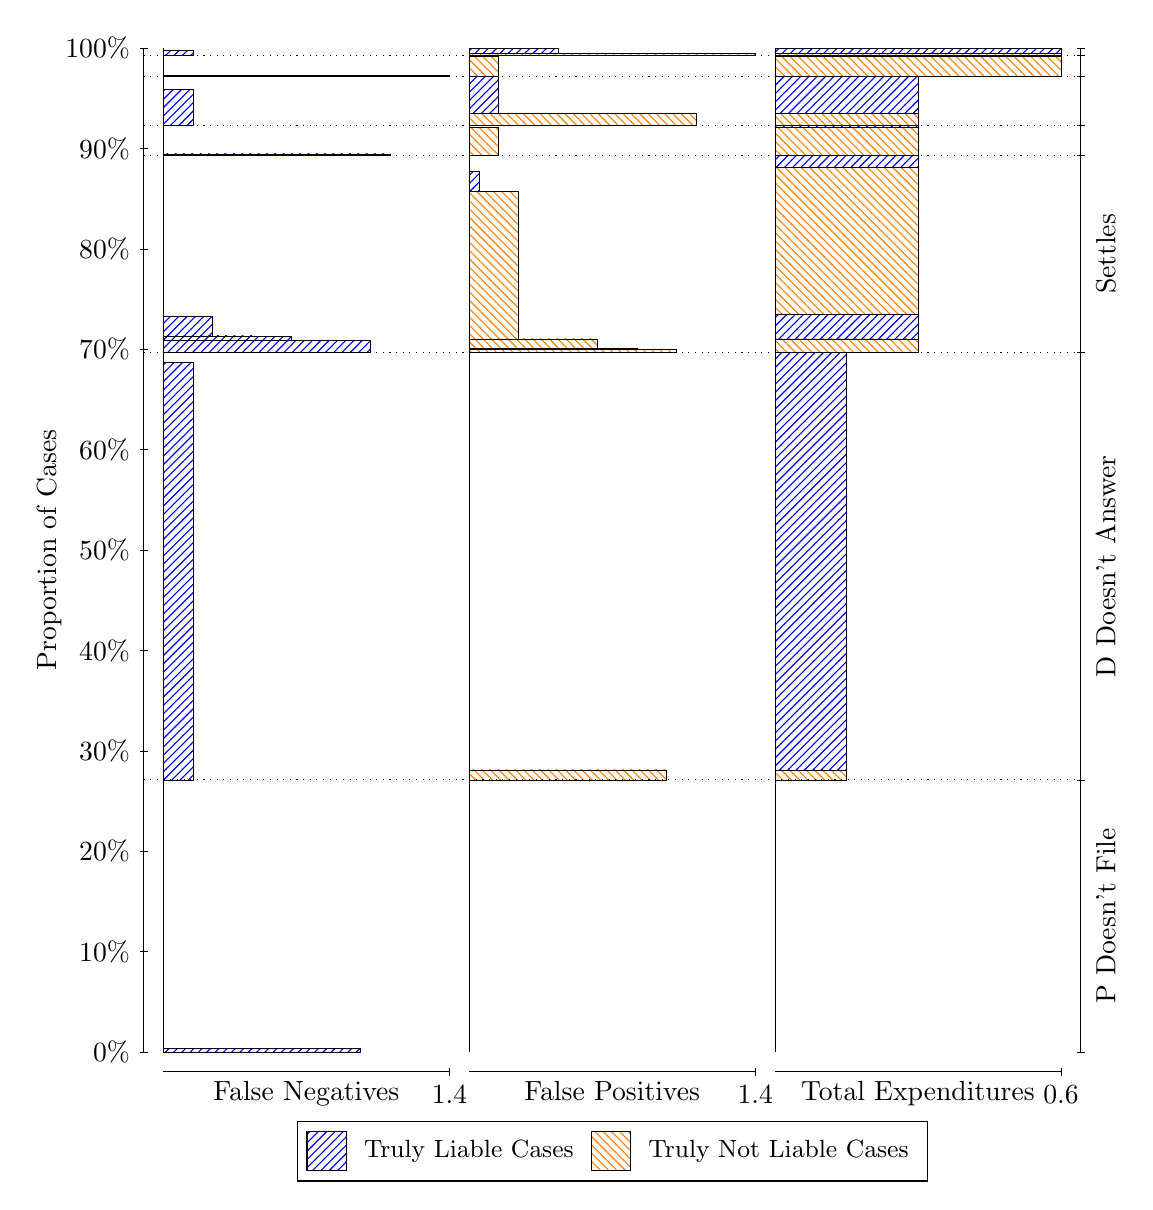
\begin{tikzpicture}
\draw[black, very thin] (1.5,1.75) -- (1.5,14.5);
\node[rotate=90, anchor=center] at (0.3, 8.125) {Proportion of Cases};
\draw[black, very thin] (1.45,1.75) -- (1.55,1.75);
\node[anchor=east] at (1.45, 1.75) {0\%};
\draw[black, very thin] (1.45,3.025) -- (1.55,3.025);
\node[anchor=east] at (1.45, 3.025) {10\%};
\draw[black, very thin] (1.45,4.3) -- (1.55,4.3);
\node[anchor=east] at (1.45, 4.3) {20\%};
\draw[black, very thin] (1.45,5.575) -- (1.55,5.575);
\node[anchor=east] at (1.45, 5.575) {30\%};
\draw[black, very thin] (1.45,6.85) -- (1.55,6.85);
\node[anchor=east] at (1.45, 6.85) {40\%};
\draw[black, very thin] (1.45,8.125) -- (1.55,8.125);
\node[anchor=east] at (1.45, 8.125) {50\%};
\draw[black, very thin] (1.45,9.4) -- (1.55,9.4);
\node[anchor=east] at (1.45, 9.4) {60\%};
\draw[black, very thin] (1.45,10.675) -- (1.55,10.675);
\node[anchor=east] at (1.45, 10.675) {70\%};
\draw[black, very thin] (1.45,11.95) -- (1.55,11.95);
\node[anchor=east] at (1.45, 11.95) {80\%};
\draw[black, very thin] (1.45,13.225) -- (1.55,13.225);
\node[anchor=east] at (1.45, 13.225) {90\%};
\draw[black, very thin] (1.45,14.5) -- (1.55,14.5);
\node[anchor=east] at (1.45, 14.5) {100\%};

\draw[black, very thin] (13.4,1.75) -- (13.4,14.5);
\draw[black, very thin] (13.35,1.75) -- (13.45,1.75);
\node[anchor=west] at (13.35, 1.75) {};
\draw[black, very thin] (13.35,5.2061) -- (13.45,5.2061);
\node[anchor=west] at (13.35, 5.2061) {};
\draw[black, very thin] (13.35,10.634) -- (13.45,10.634);
\node[anchor=west] at (13.35, 10.634) {};
\draw[black, very thin] (13.35,13.138) -- (13.45,13.138);
\node[anchor=west] at (13.35, 13.138) {};
\draw[black, very thin] (13.35,13.515) -- (13.45,13.515);
\node[anchor=west] at (13.35, 13.515) {};
\draw[black, very thin] (13.35,14.138) -- (13.45,14.138);
\node[anchor=west] at (13.35, 14.138) {};
\draw[black, very thin] (13.35,14.404) -- (13.45,14.404);
\node[anchor=west] at (13.35, 14.404) {};
\draw[black, very thin] (13.35,14.5) -- (13.45,14.5);
\node[anchor=west] at (13.35, 14.5) {};

\draw[black, very thin, pattern color=blue, pattern=north east lines] (1.75,1.75) rectangle (4.2557,1.7989);
\draw[black, very thin, pattern color=orange, pattern=north west lines] (1.75,1.7989) rectangle (1.75,5.2061);
\draw[black, very thin, pattern color=blue, pattern=north east lines] (1.75,5.2061) rectangle (2.1259,10.507);
\draw[black, very thin, pattern color=orange, pattern=north west lines] (1.75,10.507) rectangle (1.75,10.634);
\draw[black, very thin, pattern color=blue, pattern=north east lines] (1.75,10.634) rectangle (4.381,10.784);
\draw[black, very thin, pattern color=blue, pattern=north east lines] (1.75,10.784) rectangle (3.3787,10.841);
\draw[black, very thin, pattern color=blue, pattern=north east lines] (1.75,10.841) rectangle (3.1282,10.842);
\draw[black, very thin, pattern color=blue, pattern=north east lines] (1.75,10.842) rectangle (2.8776,10.843);
\draw[black, very thin, pattern color=blue, pattern=north east lines] (1.75,10.843) rectangle (2.627,10.844);
\draw[black, very thin, pattern color=blue, pattern=north east lines] (1.75,10.844) rectangle (2.3764,11.093);
\draw[black, very thin, pattern color=orange, pattern=north west lines] (1.75,11.093) rectangle (1.75,13.138);
\draw[black, very thin, pattern color=blue, pattern=north east lines] (1.75,13.138) rectangle (4.6316,13.157);
\draw[black, very thin, pattern color=orange, pattern=north west lines] (1.75,13.157) rectangle (1.75,13.515);
\draw[black, very thin, pattern color=blue, pattern=north east lines] (1.75,13.515) rectangle (2.1259,13.979);
\draw[black, very thin, pattern color=orange, pattern=north west lines] (1.75,13.979) rectangle (1.75,14.138);
\draw[black, very thin, pattern color=blue, pattern=north east lines] (1.75,14.138) rectangle (5.3833,14.153);
\draw[black, very thin, pattern color=orange, pattern=north west lines] (1.75,14.153) rectangle (1.75,14.404);
\draw[black, very thin, pattern color=blue, pattern=north east lines] (1.75,14.404) rectangle (2.1259,14.474);
\draw[black, very thin, pattern color=orange, pattern=north west lines] (1.75,14.474) rectangle (1.75,14.5);
\draw[black, very thin, pattern color=orange, pattern=north west lines] (5.6333,1.75) rectangle (5.6333,5.1571);
\draw[black, very thin, pattern color=blue, pattern=north east lines] (5.6333,5.1571) rectangle (5.6333,5.2061);
\draw[black, very thin, pattern color=orange, pattern=north west lines] (5.6333,5.2061) rectangle (8.1391,5.3339);
\draw[black, very thin, pattern color=blue, pattern=north east lines] (5.6333,5.3339) rectangle (5.6333,10.634);
\draw[black, very thin, pattern color=orange, pattern=north west lines] (5.6333,10.634) rectangle (8.2644,10.669);
\draw[black, very thin, pattern color=orange, pattern=north west lines] (5.6333,10.669) rectangle (8.0138,10.676);
\draw[black, very thin, pattern color=orange, pattern=north west lines] (5.6333,10.676) rectangle (7.7632,10.683);
\draw[black, very thin, pattern color=orange, pattern=north west lines] (5.6333,10.683) rectangle (7.5126,10.69);
\draw[black, very thin, pattern color=orange, pattern=north west lines] (5.6333,10.69) rectangle (7.2621,10.806);
\draw[black, very thin, pattern color=orange, pattern=north west lines] (5.6333,10.806) rectangle (6.2598,12.68);
\draw[black, very thin, pattern color=blue, pattern=north east lines] (5.6333,12.68) rectangle (5.7586,12.929);
\draw[black, very thin, pattern color=blue, pattern=north east lines] (5.6333,12.929) rectangle (5.6333,13.138);
\draw[black, very thin, pattern color=orange, pattern=north west lines] (5.6333,13.138) rectangle (6.0092,13.496);
\draw[black, very thin, pattern color=blue, pattern=north east lines] (5.6333,13.496) rectangle (5.6333,13.515);
\draw[black, very thin, pattern color=orange, pattern=north west lines] (5.6333,13.515) rectangle (8.5149,13.674);
\draw[black, very thin, pattern color=blue, pattern=north east lines] (5.6333,13.674) rectangle (6.0092,14.138);
\draw[black, very thin, pattern color=orange, pattern=north west lines] (5.6333,14.138) rectangle (6.0092,14.389);
\draw[black, very thin, pattern color=blue, pattern=north east lines] (5.6333,14.389) rectangle (5.6333,14.404);
\draw[black, very thin, pattern color=orange, pattern=north west lines] (5.6333,14.404) rectangle (9.2667,14.43);
\draw[black, very thin, pattern color=blue, pattern=north east lines] (5.6333,14.43) rectangle (6.7609,14.5);
\draw[black, very thin, pattern color=orange, pattern=north west lines] (9.5167,1.75) rectangle (9.5167,5.1571);
\draw[black, very thin, pattern color=blue, pattern=north east lines] (9.5167,5.1571) rectangle (9.5167,5.2061);
\draw[black, very thin, pattern color=orange, pattern=north west lines] (9.5167,5.2061) rectangle (10.425,5.3339);
\draw[black, very thin, pattern color=blue, pattern=north east lines] (9.5167,5.3339) rectangle (10.425,10.634);
\draw[black, very thin, pattern color=orange, pattern=north west lines] (9.5167,10.634) rectangle (11.333,10.806);
\draw[black, very thin, pattern color=blue, pattern=north east lines] (9.5167,10.806) rectangle (11.333,11.115);
\draw[black, very thin, pattern color=orange, pattern=north west lines] (9.5167,11.115) rectangle (11.333,12.989);
\draw[black, very thin, pattern color=blue, pattern=north east lines] (9.5167,12.989) rectangle (11.333,13.138);
\draw[black, very thin, pattern color=orange, pattern=north west lines] (9.5167,13.138) rectangle (11.333,13.496);
\draw[black, very thin, pattern color=blue, pattern=north east lines] (9.5167,13.496) rectangle (11.333,13.515);
\draw[black, very thin, pattern color=orange, pattern=north west lines] (9.5167,13.515) rectangle (11.333,13.674);
\draw[black, very thin, pattern color=blue, pattern=north east lines] (9.5167,13.674) rectangle (11.333,14.138);
\draw[black, very thin, pattern color=orange, pattern=north west lines] (9.5167,14.138) rectangle (13.15,14.389);
\draw[black, very thin, pattern color=blue, pattern=north east lines] (9.5167,14.389) rectangle (13.15,14.404);
\draw[black, very thin, pattern color=orange, pattern=north west lines] (9.5167,14.404) rectangle (13.15,14.43);
\draw[black, very thin, pattern color=blue, pattern=north east lines] (9.5167,14.43) rectangle (13.15,14.5);
\draw[black, dotted] (1.5,5.2061) -- (13.4,5.2061);
\draw[black, dotted] (1.5,10.634) -- (13.4,10.634);
\draw[black, dotted] (1.5,13.138) -- (13.4,13.138);
\draw[black, dotted] (1.5,13.515) -- (13.4,13.515);
\draw[black, dotted] (1.5,14.138) -- (13.4,14.138);
\draw[black, dotted] (1.5,14.404) -- (13.4,14.404);
\draw[black, very thin] (1.75,1.5) -- (5.3833,1.5);
\node[anchor=north] at (3.5667, 1.5) {False Negatives};
\draw[black, very thin] (5.3833,1.45) -- (5.3833,1.55);
\node[anchor=north] at (5.3833, 1.45) {1.4};

\draw[black, very thin] (5.6333,1.5) -- (9.2667,1.5);
\node[anchor=north] at (7.45, 1.5) {False Positives};
\draw[black, very thin] (9.2667,1.45) -- (9.2667,1.55);
\node[anchor=north] at (9.2667, 1.45) {1.4};

\draw[black, very thin] (9.5167,1.5) -- (13.15,1.5);
\node[anchor=north] at (11.333, 1.5) {Total Expenditures};
\draw[black, very thin] (13.15,1.45) -- (13.15,1.55);
\node[anchor=north] at (13.15, 1.45) {0.6};

\node[black, centered, rotate=90] at (13.72, 3.478) {P Doesn't File};
\node[black, centered, rotate=90] at (13.72, 7.9202) {D Doesn't Answer};
\node[black, centered, rotate=90] at (13.72, 11.886) {Settles};





\draw (7.449999999999999,1.5) node[draw=none] (baseCoordinate) {};
\begin{scope}[align=center]
        \matrix[scale=0.5, draw=black, below=0.5cm of baseCoordinate, nodes={draw}, column sep=0.1cm]{
            \node[rectangle, draw, minimum width=0.5cm, minimum height=0.5cm, pattern=north east lines, pattern color=blue] {}; &
            \node[draw=none, font=\small] (B) {Truly Liable Cases}; &
            \node[rectangle, draw, minimum width=0.5cm, minimum height=0.5cm, pattern=north west lines, pattern color=orange] {}; &
            \node[draw=none, font=\small] (B) {Truly Not Liable Cases}; \\
            };
\end{scope}

\end{tikzpicture}
\end{document}